\documentclass[twocolumn]{preport}
\usepackage[dvipdfmx]{graphicx}
\graphicspath{{figs/}}
%\verb|make pub|
\title{2018年度 中間試問 要旨 \\
空陸両用マルチリンクロータ飛行ロボットの自律移動操作行動に関する研究}
\author{稲葉・岡田研究室 指導教員 稲葉雅幸教授 \\
東京大学 工学部機械情報工学科 4 年 03170267 伊藤慶太}

\begin{document}

\pagestyle{empty}
\maketitle
\thispagestyle{empty}
\sloppy

\section{研究の背景と目的}
近年,回転翼を複数持つマルチロータ型飛行ロボットの研究が盛んに行われており,空撮や災害救助などその応用は多岐に渡る.これらの応用例の中で,本研究では物体の運搬に目を向けた.飛行ロボットによる物体運搬の特徴は,ロボットの移動が水面や起伏の激しさなどの地表面の環境に依存しないため,移動可能領域が格段に向上する点である.また,上空からの広い視野により網羅的に物体認識を行うことが可能である.その一方で,空中ではロボットの自重を支えるための揚力が必要となり,地上で物体を運搬をする場合に比べて余分にエネルギーが必要となる欠点が存在する.

そこで,本研究ではこのエネルギー効率が良くないという問題に対して,\figref{intro}(b)に示したマニピュレータ能力を持つ2次元変形ロボット"hydrus" %\cite{Hydrus:Original:2016AR}
\cite{Hydrus:Grasping:2017ICRA}が空と陸の両方の移動方法をとるアプローチにより取り組む.全体のシステム構成は\figref{intro}(a)である.はじめに物体の認識を上空から網羅的に行い,地上にて物体を把持した後,目的地までの物体運搬を周りの環境に応じて空陸の移動手段を切り替えて行うことによりエネルギー消費を抑える.

\begin{figure}[ht]
  \begin{center}
    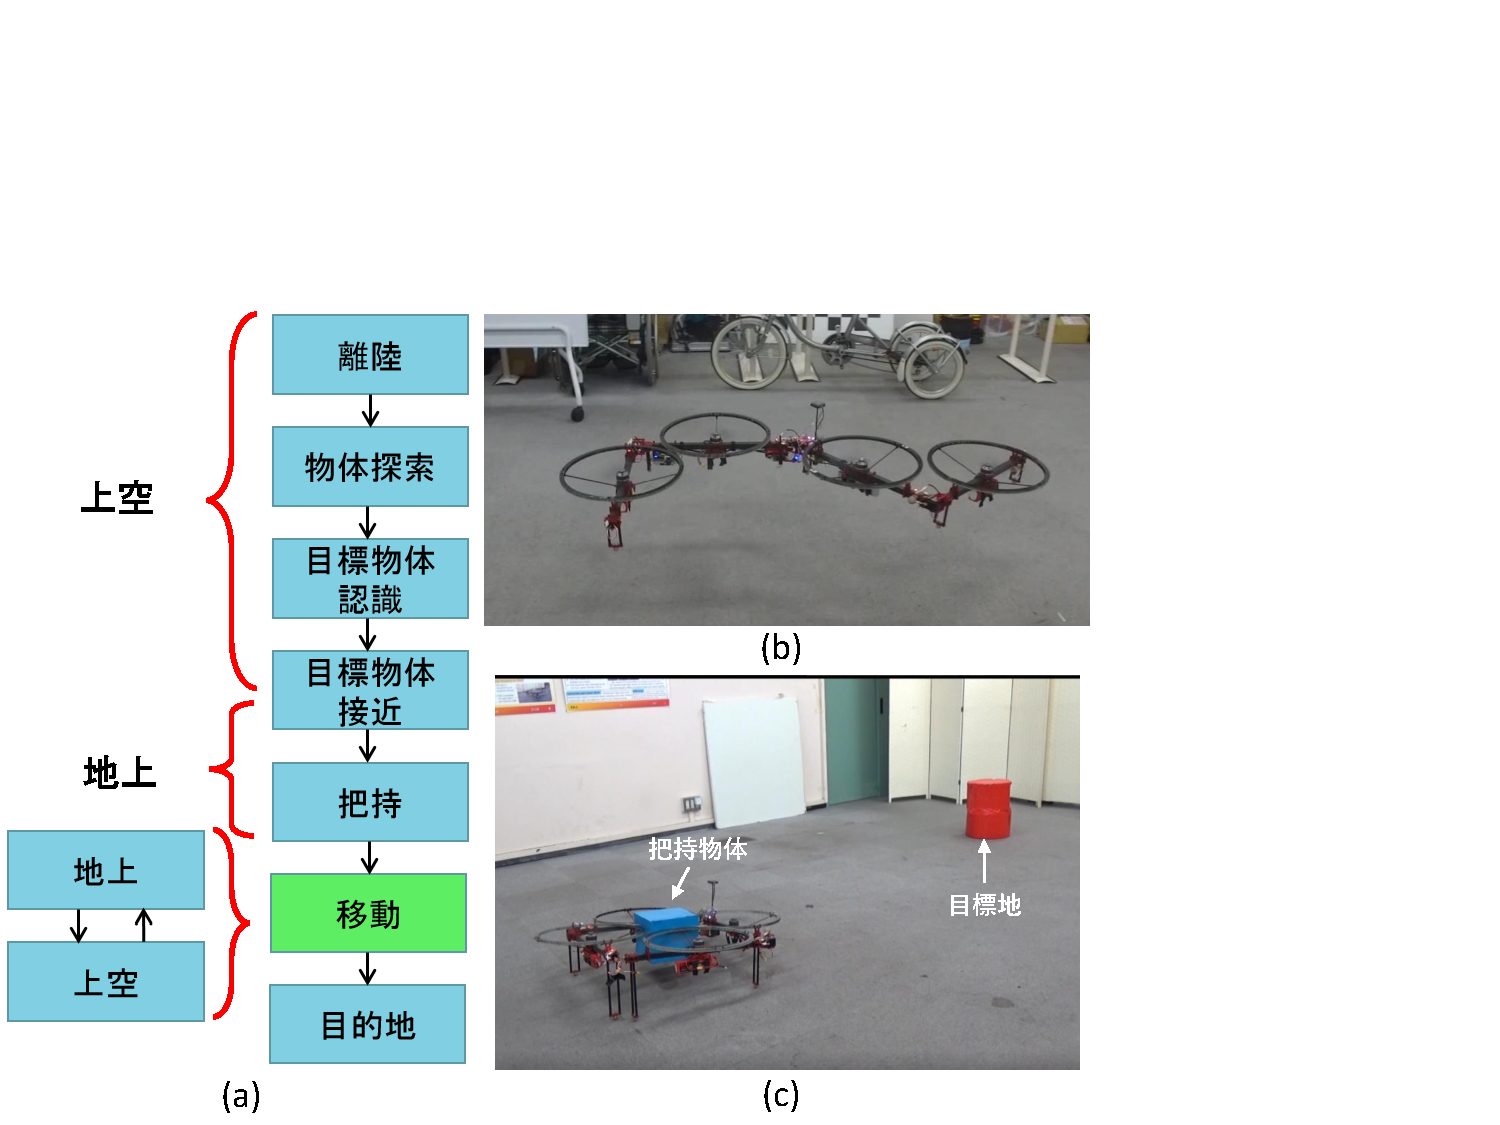
\includegraphics[clip,  bb= 0 0 526 390, width=0.85\columnwidth]{figs/intro.pdf}
  \end{center}
  \vspace{-5mm}
    \caption{(a) 全体のシステム構成,(b) hydrusが飛行する様子,(c) hydrusによる地上での物体運搬}
    \vspace{-3mm}
    \label{figure:intro}
\end{figure}

\section{現在までに行ったこと}
\subsection{目標物体の上空からの認識・地上での把持}
シュミレータ上で上空から目標物体の認識と地上での目標物体の把持ができることを確かめた.

機体に下向きに取り付けられたカメラの画像からhsi filterを用いて特定色を抽出し,そこから輪郭を抽出する.目標物体である円柱の大きさは既知として,目標物体から機体までの高さすなわち機体の地上からの高さから円柱の高さを引いた高さの情報とから,カメラの画像に写る大きさを推定し,抽出した輪郭とおよそ一致しているかどうかフィルタリングをした上で,その輪郭の中心点の座標を取得する.あとはこの座標に向けて,目標物体の周りを囲むように着地し,関節角度を変えることで目標物体を把持する,という方法を用いた.

\subsection{目的地への物体運搬}
本研究の肝となるhydrusを用いた地上での移動方法の検討・実機での検証を行った.

まず,ロボットを地上で移動させるにあたり,一般的なマルチロータ型飛行ロボットは上空でプロペラと同じ平面上を移動する際に機体を少し傾けることによりプロペラの推力の水平成分を生み出し移動している点に注目し,機体が傾いた状態で地面に接地するように改良を施すことを考えた.これは\figref{ground_mode}(a)で示しているように先端にボールキャスターの付いた長さの異なる足を数カ所機体に取り付けることで実現した.

\begin{figure}[ht]
  \begin{center}
    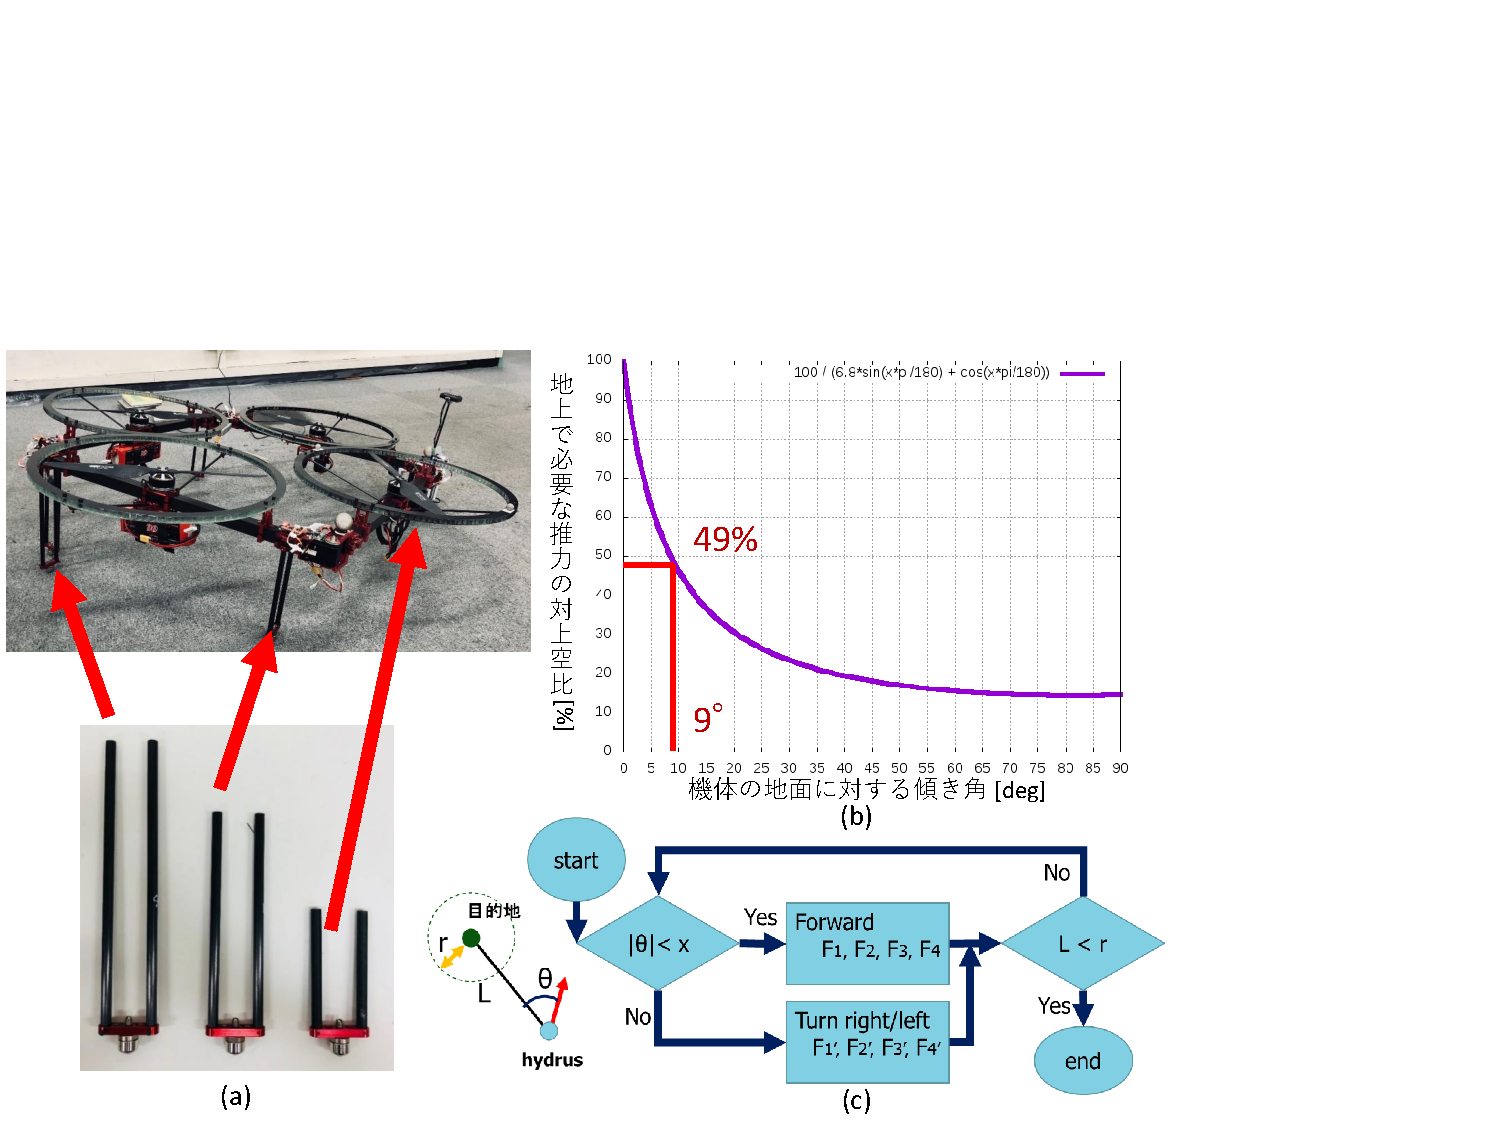
\includegraphics[clip,  bb= 0 0 564 374, width=0.9\columnwidth]{figs/ground_motion.pdf}
  \end{center}
  \vspace{-5mm}
    \caption{(a) 機体の傾け方,(b) 機体の傾き角と地上での移動に必要な推力の対上空比の関係,(c) 地上での移動の制御方法}
%    \vspace{-3mm}
    \label{figure:ground_mode}
\end{figure}


次に,どのような制御方法により目的地までhydrusが地上を走行していくかを考えた.本研究が目指しているのは厳密な経路追従ではなく目的地への到達である点を考慮し,キャスターと地面との摩擦を考慮したモデルベースの制御をせずに,地上での動きを前進・右折・左折の3パターンに絞り,それらのパターンの繰り返しにより目的地に向かうことを考えた.それぞれの動きは4つのプロペラに一定の推力すなわち回転数を与えることで実現した.この推力は事前に人が調整を行った値をパラメータとして保存したものである.そして,ロボットの目的地に対する姿勢と目的地までの距離を\figref{ground_mode}(c)に示したループにより制御した.

実機での検証では,\figref{intro}(c)のようにhydrusが赤い円柱の物体を目的地として搭載されたカメラで認識し,地上を走行して到達できることを示せた.ロボットの位置と姿勢を得るのにはモーションキャプチャを用いている.また,理論式から導き出された\figref{ground_mode}(b)の通り,上空移動に必要な推力の半分で移動できることを示せた.

\if 0
\begin{figure}[ht]
  \begin{center}
    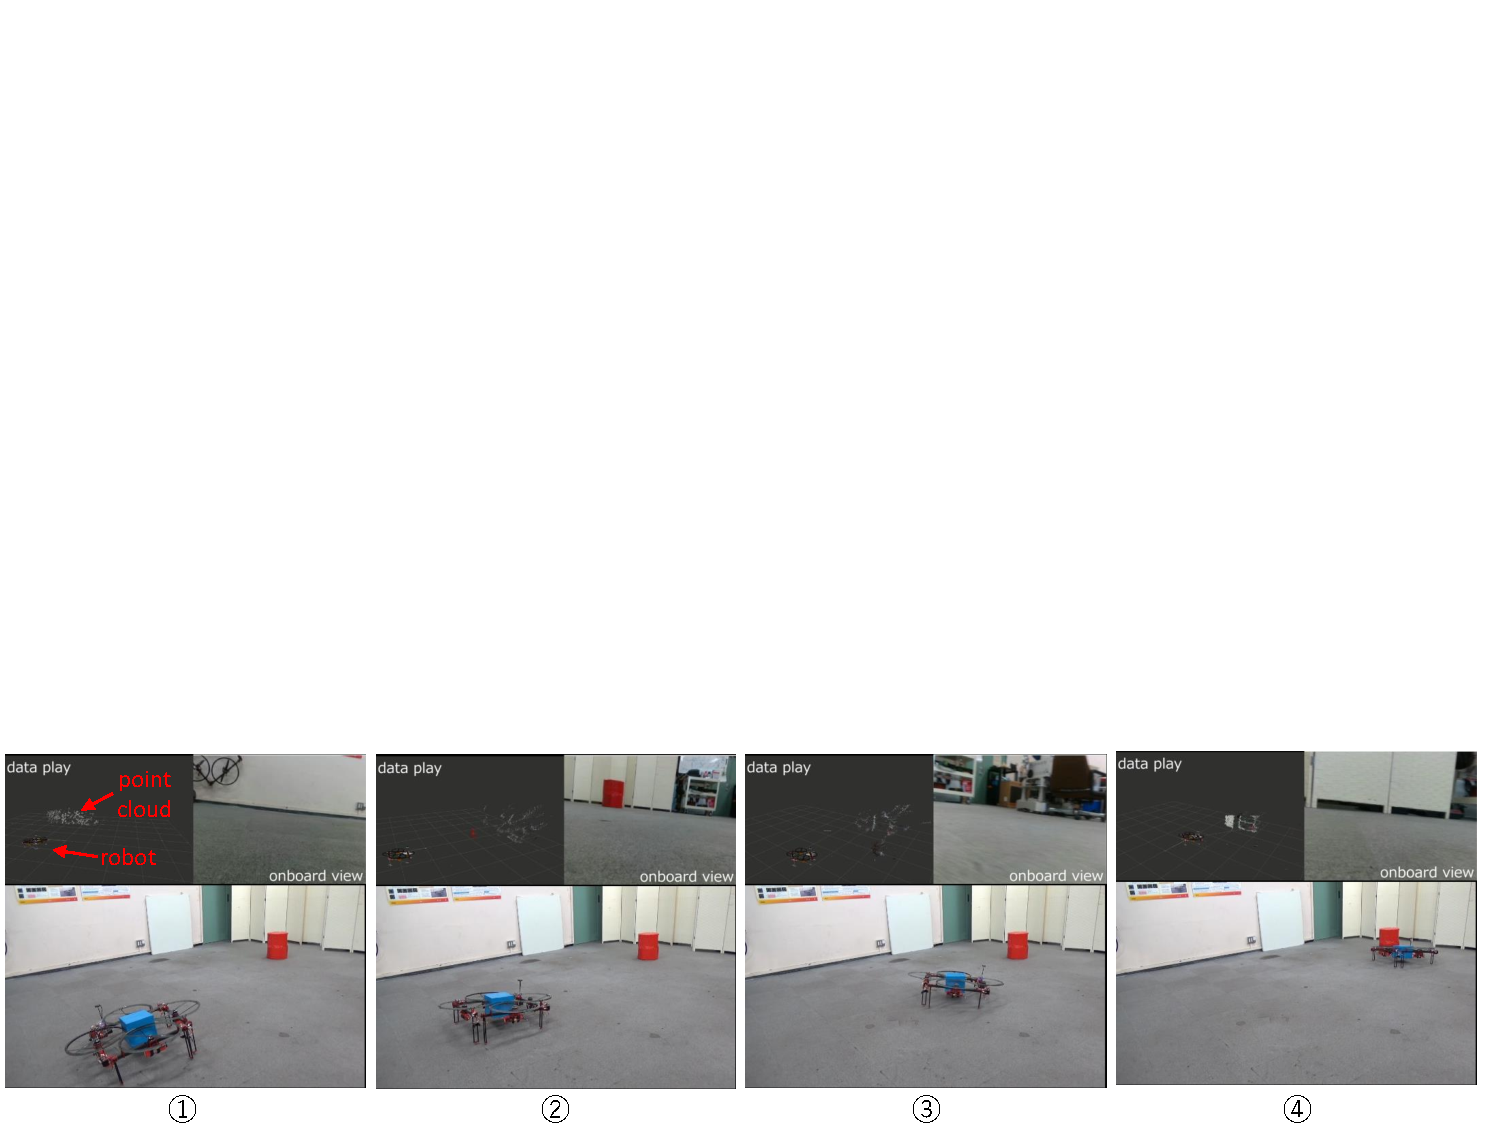
\includegraphics[clip,  bb= 0 0 711 180, width=1.0\columnwidth]{figs/go-marker.pdf}
  \end{center}
  \vspace{-5mm}
  \caption{The moton sequence of go marker}
      \vspace{-3mm}
  \label{figure:go_marker}
\end{figure}
\fi

\section{考察と今後の指針}
現段階で上空移動に必要な推力の半分で移動可能であることは示せたが,移動速度の観点から見るとエネルギー効率が向上したと断定するには早く,上空移動との比較を移動速度の観点にも目を向けながら研究を進めていきたい.

このことを踏まえた上で今後の研究指針としては,ロボットの自律移動操作行動を可能にするために,強化学習により地上での移動に関する各プロペラの推力などのパラメータ調整を自動化することや,地上で物体運搬する際に物体が地面に擦らないようにするための機体の改良,そして地上の環境に応じた動的な移動方式の選択方法の検討が考えられる.

\bibliographystyle{junsrt}
\bibliography{p-report}

\end{document}

